\documentclass[aspectratio=169,11pt]{beamer}
\usepackage[T1]{fontenc}
\usepackage{lmodern,amsmath,amssymb,mathtools,bm,booktabs,array,graphicx,tikz}
\usetikzlibrary{arrows.meta,positioning,calc,decorations.pathreplacing,patterns}
\definecolor{ink}{HTML}{17344D}\definecolor{accent}{HTML}{087E8B}\definecolor{pale}{HTML}{EDF5F5}\definecolor{gold}{HTML}{AD6B19}
\providecommand{\dd}{\,\mathrm{d}}\providecommand{\R}{\mathbb{R}}
\providecommand{\E}{\mathbb{E}}\providecommand{\Var}{\operatorname{Var}}
\providecommand{\Cov}{\operatorname{Cov}}\providecommand{\diag}{\operatorname{diag}}
\providecommand{\norm}[1]{\left\lVert#1\right\rVert}
\providecommand{\abs}[1]{\left|#1\right|}
\usefonttheme{professionalfonts}
\setbeamercolor{normal text}{fg=black,bg=white}
\setbeamercolor{frametitle}{fg=ink,bg=white}
\setbeamercolor{title}{fg=ink}\setbeamercolor{structure}{fg=accent}
\setbeamercolor{block title}{fg=ink,bg=pale}\setbeamercolor{block body}{fg=black,bg=pale!40}
\setbeamercolor{alerted text}{fg=accent}
\setbeamerfont{frametitle}{size=\Large,series=\bfseries}
\setbeamerfont{title}{size=\LARGE,series=\bfseries}
\setbeamertemplate{navigation symbols}{}
\setbeamersize{text margin left=.7cm,text margin right=.7cm}
\setbeamertemplate{frametitle}{\vspace{.18cm}\insertframetitle\par\vspace{.1cm}{\color{accent}\hrule height .6pt}\vspace{.12cm}}
\newcommand{\notestarget}{notes.pdf}\newcommand{\noteslabel}{Notes}
\setbeamertemplate{footline}{\hspace{.7cm}\color{ink}\scriptsize Mathematical Modeling\quad\href{\notestarget}{\noteslabel}\hfill\insertframenumber\,/\,\inserttotalframenumber\hspace{.7cm}\vspace{.18cm}}
\setbeamercovered{invisible}
\hypersetup{pdfauthor={Zan Ahmad},pdftitle={Crossbridge populations: transition kinetics and mechanical force},pdfpagemode=UseNone}
\begin{document}
\begin{frame}[plain]\vfill
{\small\color{accent} Mathematical Modeling \quad Lecture 5}\par\medskip
{\raggedright\hyphenpenalty=10000\exhyphenpenalty=10000\LARGE\bfseries\color{ink} Crossbridge populations: transition kinetics and mechanical force}\par\bigskip
Zan Ahmad\par\smallskip
{\small Fall 2024}\par\vfill\end{frame}
\renewcommand{\notestarget}{notes.pdf\#note-a-two-state-description-of-crossbridge-occupancy}
\begin{frame}[t,fragile,label=slide-attached-and-detached-populations]{Attached and detached populations}
$A+D=1$, with $A,D\in[0,1]$.\par\medskip A fixed population of heads changes category; filaments slide relative to one another.\pause{}\par\medskip Occupancy retains chemical state but discards displacement.
\end{frame}
\renewcommand{\notestarget}{notes.pdf\#note-conservation-and-the-transition-generator}
\begin{frame}[label=slide-transition-fluxes-figure]{Transition fluxes}
\centering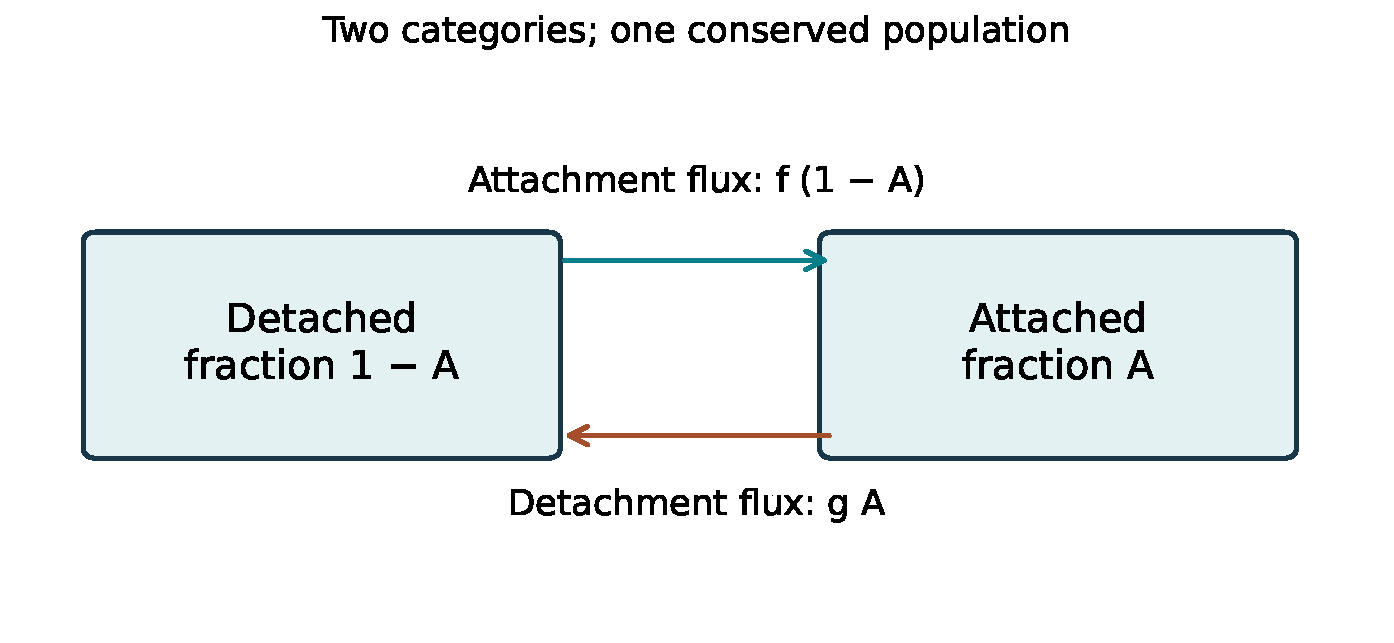
\includegraphics[width=.98\linewidth,height=.69\textheight,keepaspectratio]{state-balance.pdf}\end{frame}
\renewcommand{\notestarget}{notes.pdf\#note-conservation-and-the-transition-generator}
\begin{frame}[t,fragile,label=slide-transition-fluxes]{Transition fluxes}
\[J_{D\to A}=fD,\qquad J_{A\to D}=gA.\]\pause{} $[f]=[g]=\mathrm{s}^{-1}$; both fluxes are population fraction per second.\par\medskip A transition requires a head in its source category.
\end{frame}
\renewcommand{\notestarget}{notes.pdf\#note-conservation-and-the-transition-generator}
\begin{frame}[t,fragile,label=slide-the-conserved-two-state-system]{The conserved two-state system}
\[\frac{\dd}{\dd t}\binom D A=\begin{pmatrix}-f&g\\f&-g\end{pmatrix}\binom D A.\]\pause{}\[\dot D+\dot A=0,\qquad \dot A=f-(f+g)A.\]
\end{frame}
\renewcommand{\notestarget}{notes.pdf\#note-conservation-and-the-transition-generator}
\begin{frame}[t,fragile,label=slide-invariant-fraction-interval]{Invariant fraction interval}
\[\dot A\big|_{A=0}=f\geq0,\qquad \dot A\big|_{A=1}=-g\leq0.\]\pause{} The vector field points into the admissible interval at both endpoints.\par\medskip A negative computed fraction is not an alternative biological state.
\end{frame}
\renewcommand{\notestarget}{notes.pdf\#note-equilibrium-relaxation-and-rate-identification}
\begin{frame}[t,fragile,label=slide-equilibrium-with-continuing-turnover]{Equilibrium with continuing turnover}
\[f(1-A_\infty)=gA_\infty\quad\Longrightarrow\quad A_\infty=\frac f{f+g}.\]\pause{} For $f=3$, $g=1\,\mathrm{s}^{-1}$:\[A_\infty=0.75,\qquad J_{D\to A}=J_{A\to D}=0.75\,\mathrm{s}^{-1}.\]
\end{frame}
\renewcommand{\notestarget}{notes.pdf\#note-equilibrium-relaxation-and-rate-identification}
\begin{frame}[t,fragile,label=slide-derivation-of-the-relaxation-law]{Derivation of the relaxation law}
\[\frac{\dd}{\dd t}(A-A_\infty)=-(f+g)(A-A_\infty).\]\pause{}\[A(t)=A_\infty+(A_0-A_\infty)e^{-t/\tau},\qquad\tau=(f+g)^{-1}.\]
\end{frame}
\renewcommand{\notestarget}{notes.pdf\#note-equilibrium-relaxation-and-rate-identification}
\begin{frame}[label=slide-endpoint-and-timescale-identify-different-parameters-figure]{Endpoint and timescale identify different parameters}
\centering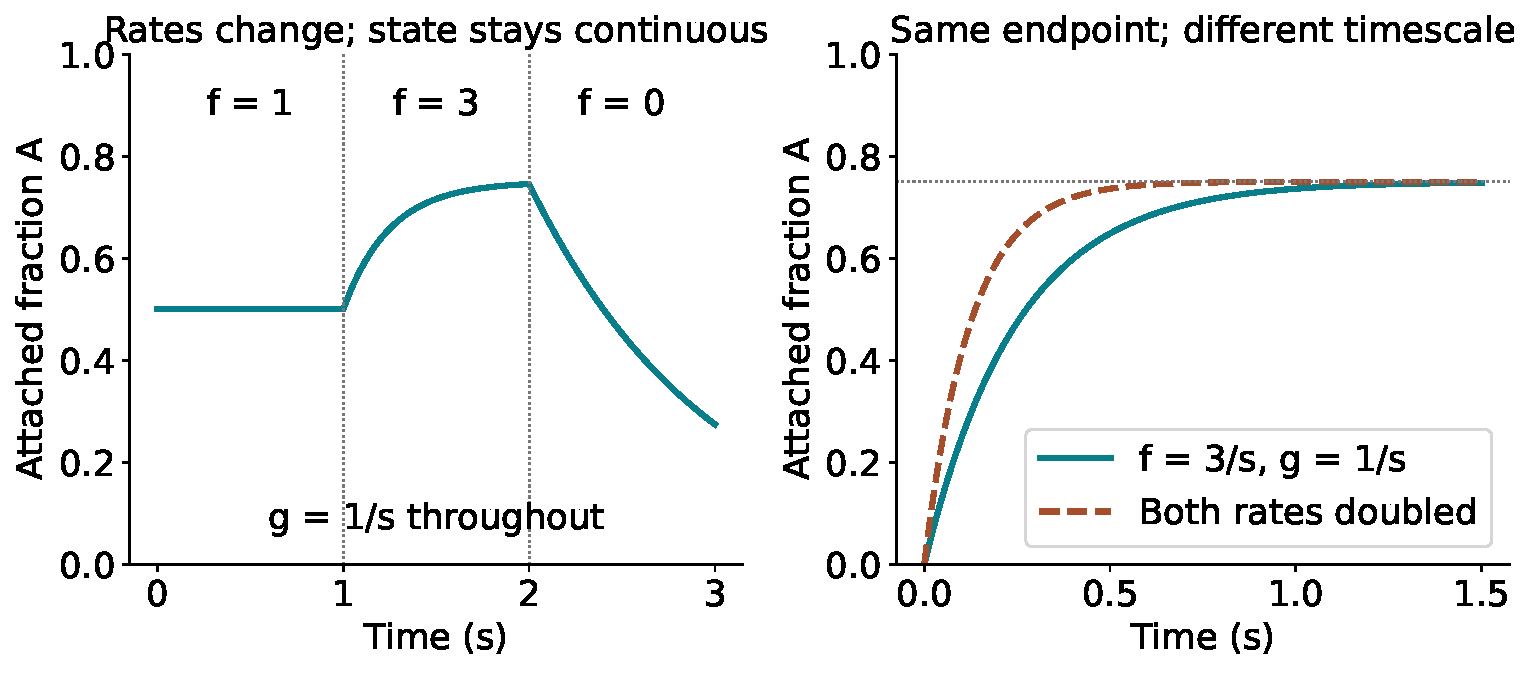
\includegraphics[width=.98\linewidth,height=.69\textheight,keepaspectratio]{occupancy-traces.pdf}\end{frame}
\renewcommand{\notestarget}{notes.pdf\#note-equilibrium-relaxation-and-rate-identification}
\begin{frame}[t,fragile,label=slide-endpoint-and-timescale-identify-different-parameters]{Endpoint and timescale identify different parameters}
\[(f,g)\mapsto(cf,cg):\qquad A_\infty\mapsto A_\infty,\quad\tau\mapsto\tau/c.\]\pause{}\[f=A_\infty/\tau,\qquad g=(1-A_\infty)/\tau.\] An endpoint alone cannot identify both rates.
\end{frame}
\renewcommand{\notestarget}{notes.pdf\#note-rate-changes-and-numerical-preservation-of-fractions}
\begin{frame}[t,fragile,label=slide-exact-updates-across-rate-switches]{Exact updates across rate switches}
\[A_{n+1}=A_\infty+(A_n-A_\infty)e^{-(f+g)h}.\]\pause{} Carry $A_{n+1}$ into the next interval.\par\medskip A rate switch changes the slope, not the current attached fraction.
\end{frame}
\renewcommand{\notestarget}{notes.pdf\#note-rate-changes-and-numerical-preservation-of-fractions}
\begin{frame}[t,fragile,label=slide-a-three-stage-calculation]{A three-stage calculation}
\[\begin{aligned}A(1)&=0.5,\\A(2)&=0.75-0.25e^{-4}\simeq0.74542,\\A(3)&=A(2)e^{-1}\simeq0.27422.\end{aligned}\]\pause{} Attachment is first balanced, then increased, then switched off.
\end{frame}
\renewcommand{\notestarget}{notes.pdf\#note-rate-changes-and-numerical-preservation-of-fractions}
\begin{frame}[t,fragile,label=slide-euler-accuracy-and-admissibility]{Euler accuracy and admissibility}
\[A_{n+1}=A_n+h\{f(1-A_n)-gA_n\}.\]\pause{} $A_n=0.5$, $f=3$, $g=1$, $h=0.05$ gives $0.55$; exact: $0.54532$.\par\medskip $hf\leq1$ and $hg\leq1$ preserve $[0,1]$; smaller steps may still be needed for accuracy.
\end{frame}
\renewcommand{\notestarget}{notes.pdf\#note-rate-changes-and-numerical-preservation-of-fractions}
\begin{frame}[t,fragile,label=slide-the-zero-rate-and-one-way-limits]{The zero-rate and one-way limits}
\[\begin{array}{c|c}f=g=0&A(t)=A_0\\f=0,\ g>0&A(t)=A_0e^{-gt}\\g=0,\ f>0&A(t)=1-(1-A_0)e^{-ft}\end{array}\]
\end{frame}
\renewcommand{\notestarget}{notes.pdf\#note-mechanical-force-requires-a-distribution-or-a-closure}
\begin{frame}[t,fragile,label=slide-a-fixed-force-closure]{A fixed-force closure}
\[F=NAF_{\mathrm{head}}.\]\pause{}\[1000\times0.75\times2\,\mathrm{pN}=1.5\,\mathrm{nN}.\] All attached heads are assumed to exert the same aligned force.
\end{frame}
\renewcommand{\notestarget}{notes.pdf\#note-mechanical-force-requires-a-distribution-or-a-closure}
\begin{frame}[t,fragile,label=slide-occupancy-and-force-are-different-moments]{Occupancy and force are different moments}
\[A=\int u(x,t)\,\dd x,\qquad F=N\int p(x)u(x,t)\,\dd x.\]\pause{} If $p(x)=\kappa x$, equal attached fractions may have different mean strains and different forces.
\end{frame}
\renewcommand{\notestarget}{notes.pdf\#note-mechanical-force-requires-a-distribution-or-a-closure}
\begin{frame}[t,fragile,label=slide-reduction-of-a-displacement-model]{Reduction of a displacement model}
\[\partial_tu-v\partial_xu=f(1-A)\delta(x-x_a)-gu.\]\pause{} Integrate over displacement, with vanishing endpoint flux:\[\dot A=f(1-A)-gA.\]
\end{frame}
\renewcommand{\notestarget}{notes.pdf\#note-computation-and-the-scope-of-a-force-measurement}
\begin{frame}[t,fragile,label=slide-rate-experiments-in-the-companion]{Rate experiments in the companion}
Compare $(f,g)=(3,1)$ and $(6,2)$.\par\medskip Check exact interval composition, fraction bounds, and pure detachment.\pause{}\par\medskip Report endpoint, relaxation time, and the assumed force per head separately.
\end{frame}
\renewcommand{\notestarget}{notes.pdf\#note-computation-and-the-scope-of-a-force-measurement}
\begin{frame}[t,fragile,label=slide-mechanical-and-chemical-power]{Mechanical and chemical power}
\[P_{\mathrm{mechanical}}=Fv.\]\pause{} At $v=0$, force and transition fluxes may remain nonzero.\par\medskip ATP consumption requires chemical stoichiometry and free energy per cycle.
\end{frame}
\end{document}
